\newchapter{Uruchomienie projektu}{Grzegorz Wąs}
\label{app:app1}

    \section{Spis zawartości dołączonej płyty CD}

        Zawartość dołączonej do niniejszej pracy płyty CD przedstawia się następująco:

        \begin{itemize}
            \item \texttt{access-control-system} - główny katalog projektu
                \begin{itemize}
                    \item \texttt{controller} - katalog z oprogramowaniem mikrokontrolera
                    \item \texttt{management} - katalog z oprogramowaniem zarządzajacym
                    \item \texttt{server} - katalog z oprogramowaniem autoryzującym
                \end{itemize}
                \item \texttt{vagrantfile} - plik narzędzia Vagrant
        \end{itemize}

        Struktura plików każdego z wyżej wymienionych katalogów została przedstawiona na rysunkach \ref{fig:controller_katalogi} (projekt oprogramowania układu zamka), \ref{fig:zarzadzanie_katalogi} (projekt oprogramowania podsystemu zarządzania) oraz \ref{fig:serwer_katalogi} (projekt oprogramowania podsystemu autoryzacji).

    \begin{figure}[]
        \centering
        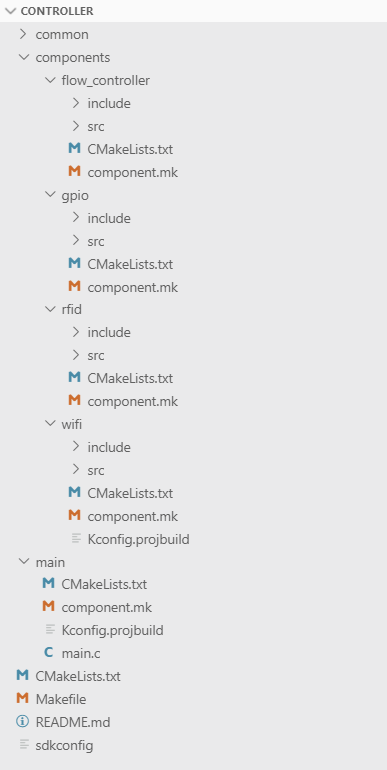
\includegraphics[width=0.5\textwidth]{chapters/images/struktura_katalogow.png}
        \caption{Struktura plików projektu oprogramowania układu zamka}
        \label{fig:controller_katalogi}
    \end{figure}

    \begin{figure}[]
        \centering
        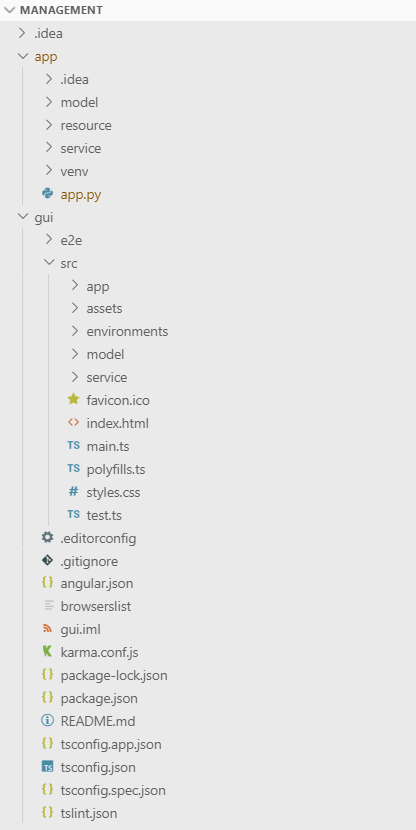
\includegraphics[width=0.5\textwidth]{chapters/images/struktura_katalogow_mngmt.png}
        \caption[{Struktura plików projektu systemu zarządzania}]{Struktura plików projektu systemu zarządzania, app - aplikacja API, gui - aplikacja GUI}
        \label{fig:zarzadzanie_katalogi}
    \end{figure}

    \begin{figure}[]
        \centering
        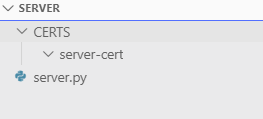
\includegraphics[width=0.5\textwidth]{chapters/images/struktura_katalogow_serwer.png}
        \caption{Struktura plików projektu oprogramowania podsystemu autoryzacji}
        \label{fig:serwer_katalogi}
    \end{figure}

\section{Oprogramowanie kontrolera}

    \subsection{Wymagania wstępne}
    Środowisko uruchomienia projektu musi spełniać następujące wymagania:
    \begin{itemize}
        \item połączenie z internetem - narzędzia wykorzystywane do zarządzania projektem udostępniane są jako repozytoria systemu kontroli wersji git lub pakiety dostępne za pośrednictwem narzędzia \texttt{apt-get},
        \item oprogramowanie VirtualBox - środowisko deweloperskie stworzone zostało w oparciu maszynę wirtualną z systemem operacyjnym typu Linux Ubuntu,
        \item oprogramowanie Vagrant - narzędzie wykorzystywane w celu uproszczenia i automatyzacji procesu wdrożenia środowiska deweloperskiego. Pozwala spójnie zdefiniować proces wdrożenia, zaczynając od stworzenia maszyny wirtualnej, przez konfigurację interfejsów sieciowych, aż po konfigurację systemu operacyjnego i aplikacji.
    \end{itemize}

    \subsection{Instrukcja konfiguracji środowiska}
        Aby skonfigurować środowisko w celu utrzymania i rozwoju projektu, należy wykonać następujące kroki:
        \begin{enumerate}
            \item Utworzyć na dysku katalog \texttt{PROJEKT}, gdzie \texttt{PROJEKT} to dowolna poprawna nazwa.
            \item Przenieść zawartość płyty do katalogu \texttt{PROJEKT}.
            \item Uruchomić terminal w katalogu \texttt{PROJEKT}.
            \item Wykonać polecenie \texttt{vagrant up} (wykonanie polecenia może trwać około 30 minut).
        \end{enumerate}

        Powyższe kroki sktukują utworzeniem maszyny wirtualnej z zainstalowanym zestawem narzędzi potrzebnych do uruchomienia projektu. Aby uruchomić tę maszynę, w folderze \texttt{PROJEKT} wywołać komendę \texttt{vagrant ssh}. Spowoduje to wyświetlenie tekstowego interfejsu nowo utworzonej maszyny wirtualnej. Aby uruchomić projekt należy:

        \begin{enumerate}
            \item Przejść do katalogu \texttt{\~{}/esp/controller}.
            \item Podłączyć układ zamka poprzez interfejs USB.
            \item Wywołać komendę \texttt{esp.idf menuconfig} - spowoduje to wyświetlenie menu tekstowego umożliwiającego konfigurację mikrokontrolera. W menu \texttt{Wifi configuration} znajdują się opcje pozwalające na konfigurację parametrów takich jak adres IP serwera, port serwera, nazwa sieci WiFi, hasło sieci WiFi. W menu \texttt{General controller configuration} znajduje się opcja umożliwiająca ustawienie ID zamka.
            \item Wywołać komendę \texttt{idf.py -p PORT\_USB flash monitor}, gdzie \texttt{PORT\_USB} to np. \texttt{/dev/ttyUSB0}. Dodanie opcji \texttt{monitor} umożliwia odczytywanie logów mikrokontrolera poprzez port szeregowy.
        \end{enumerate}

        Uwaga: Domyślnie zarówno kontroler jak i serwer wykorzystują predefiniowane certyfikaty. Aby osiągnąc odpowiedni poziom bezpieczeństwa należy wygenerować certyfikaty na nowo.

        Na rysunkach \ref{fig:men1} i \ref{fig:men2} przedstawiono odpowiednio: wygląd głównego menu narzędzia \texttt{menuconfig} oraz wygląd submenu o nazwie \texttt{Wifi configuration}.

        \begin{figure}[]
            \centering
            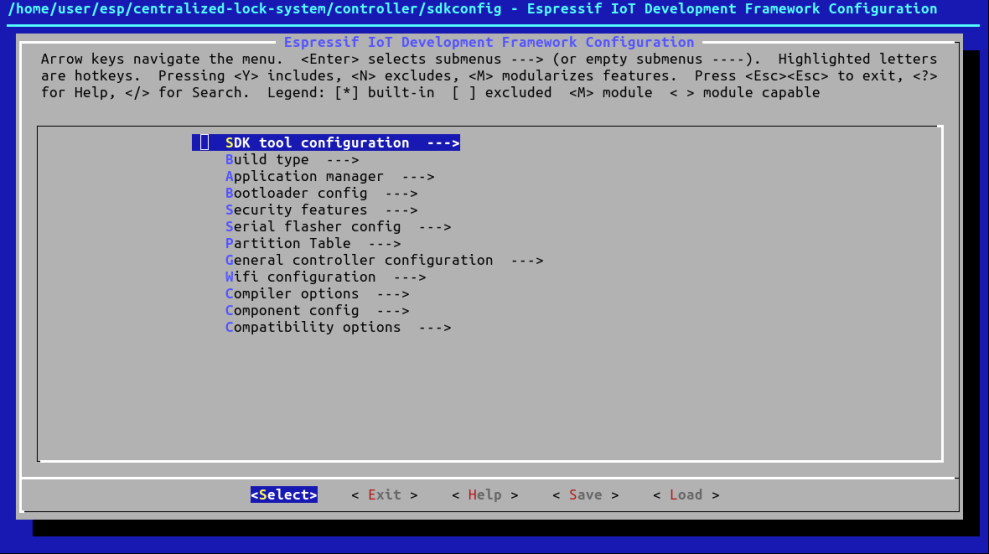
\includegraphics[width=\textwidth]{chapters/images/menuconfig1.png}
            \caption{Widok głównego menu \texttt{menuconfig}}
            \label{fig:men1}
        \end{figure}

        \begin{figure}[]
            \centering
            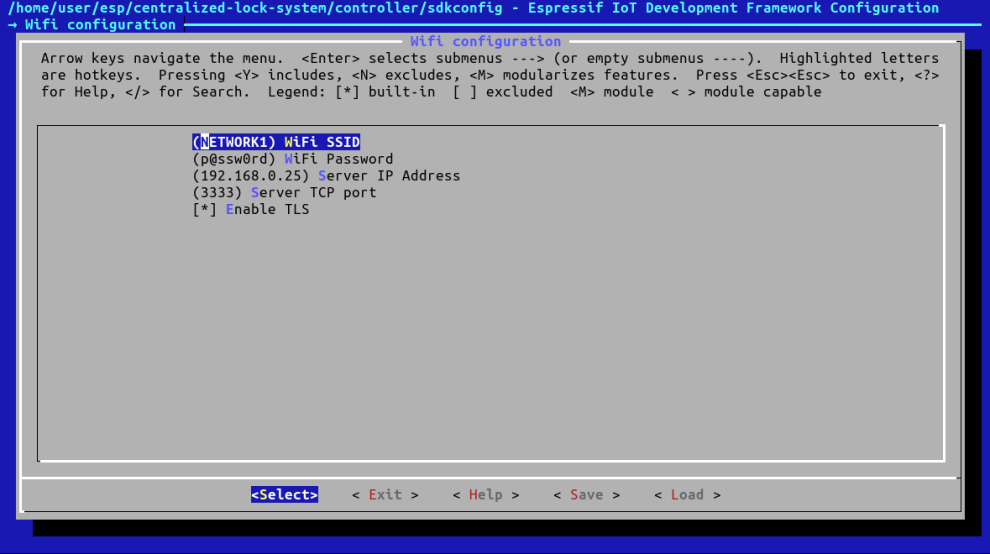
\includegraphics[width=\textwidth]{chapters/images/menuconfig2.png}
            \caption{Widok submenu \texttt{Wifi configuration}}
            \label{fig:men2}
        \end{figure}

\section{Oprogramowanie autoryzujące}
    Jedynym wymaganiem wobec środowiska uruchomienia oprogramowania autoryzującego jest dostępność interpretera języka Python i dostęp sieci bezprzewodowej, poprzez którą będzie się odbywała komunikacja z układem zamka.
    W celu uruchomienia oprogramowania serwera należy serwera uruchomić terminal w katalogu \texttt{access-control-system/server} i wywołać komendę \texttt{python server.py}.

\section{Oprogramowanie zarządzające}

\subsection{Aplikacja API}
        Środowisko uruchomienia aplikacji API oprogramowania zarządzającego do działania wymaga jedynie interpretera języka Python z zainstalowanym modułem Flask. W celu uruchomienia aplikacji należy przejść do katalogu \texttt{access-control-system/management/app} i wywołać komendę \texttt{python app.py}.

\subsection{Aplikacja GUI}
        Do uruchomienia projektu potrzebne jest zintegrowane środowisko deweloperskie Intellij IDEA Ultimate firmy JetBrains. Po otworzeniu projektu w środowisku należy uruchomić go poprzez kliknięcie na ikonę zielonej strzałki.

Aplikacje zostały skonfigurowane w sposób umożliwiający im komunikację za pomocą wewnętrznego interfejsu sieciowego \textit{localhost}.



